\documentclass[a4paper]{article}

\usepackage{graphicx}
\usepackage{float}
\usepackage{listings}
\usepackage{color}

\definecolor{dkgreen}{rgb}{0,0.6,0}
\definecolor{gray}{rgb}{0.5,0.5,0.5}
\definecolor{mauve}{rgb}{0.58,0,0.82}

\lstset{frame=tb,
  language=Python,
  aboveskip=3mm,
  belowskip=3mm,
  showstringspaces=false,
  columns=flexible,
  basicstyle={\small\ttfamily},
  numbers=none,
  numberstyle=\tiny\color{gray},
  keywordstyle=\color{blue},
  commentstyle=\color{dkgreen},
  stringstyle=\color{mauve},
  breaklines=true,
  breakatwhitespace=true,
  tabsize=3
}

\begin{document}



\begin{enumerate}
    \item \begin{enumerate}
        \item Elmo - $94*10^6$, Jan 2018,  https://allennlp.org/elmo, \\ \\
              GPT-2 - $1,5*10^9$, Feb 2019, https://openai.com/blog/gpt-2-1-5b-release/ \\ \\
              Megatron-LM, $8,3*10^9$, Mar 2019,https://www.deepspeed.ai/tutorials/megatron/ \\ \\
              Turing-NLG- $17*10^9$, Feb 2020, https://www.microsoft.com/en-us/research/blog/turing-nlg-a-17-billion-parameter-language-model-by-microsoft/ \\ \\
              GPT-3 $175*10^9$, Juni 2020, https://openai.com/blog/openai-api/ \\ \\
              Megatron-Turing-NLG - , $530*10^9$,October 2021, https://developer.nvidia.com/blog/using-deepspeed-and-megatron-to-train-megatron-turing-nlg-530b-the-worlds-largest-and-most-powerful-generative-language-model/  \\ \\ 
              All of these are taken from the website of the company that created them. And thus we can be sure the data is correct. See table 1.
            \item See figure 1.
            \item The amount of months after the start of 2018 as our x value and log parameters as our y value. See table 2.
            \item See figure 2. 
            \item No we can not see any visual outliers. 

    \end{enumerate}
    \item \begin{enumerate}
        \item  $z^x$ exponential function
        $log(z)^x = x * log(z)$ linear function
        We require a linear function for the regression model which is why the y variable is logarithmic.
        \item Running code seen in code example we get $\alpha =0.08427335479400888$ and $\beta = 8.190329535314607$
        \item See figure 2c.
        \item See figure 2d. 
        \item Did not understand question. 
        \item One step would be a step of 10. So to solve this we would solve $1*x = \beta$ which is the same as $x = 1/\beta$. Which is roughly $11.866$. 
    \end{enumerate}
    \item \begin{enumerate}
        \item H0 : beta = 0.
        H1: beta != 0. 
        If zero is included in our interval we know there is no linear relation. See our calculations. We get the interval to [0.049654, 0.11888]. As zero is not included in this interval we can discard H0 and say that we have a significant linear correlation.
         
        \item Here we need 1/limits from question 3a. Which gives us: [8.41184, 20.139] 
        \item This question has been done on paper see figure 6. 
        \item  No I do not think so. This regression curve is based on a small set of data and therefor will have a hard time predicting far into the future. 
    \end{enumerate}
\end{enumerate}

\section*{Code}
\begin{lstlisting}
    #Code for 2b
    import math

    x = [1,14,15,26,30,46]
    y = [math.log10(94 *10**6),
         math.log10(1.5*10**9),
         math.log10(8.3*10**9),
         math.log10(17 *10**9),
         math.log10(175*10**9),
         math.log10(530*10**9)]
    
    def average(list):
        total = 0
        for i in range(len(list)):
            total += list[i]
        return (total / len(list))
    
    x_average = average(x)
    y_average = average(y)
    
    def calc_s (list1,list2,average1,average2):
        total = 0
        for i in range(len(list1)):
            total += (list1[i]-average1)*(list2[i]-average2)
        return total
    
    sxx = calc_s(x,x,x_average,x_average)
    syy = calc_s(y,y,y_average,y_average)
    sxy = calc_s(x,y,x_average,y_average)
    
    BHat = sxy/sxx
    alpha = y_average - x_average*BHat
    
    print(BHat)
    print(alpha)
    \end{lstlisting}

\section*{Graphs and tables:}
              \begin{table}[h]
                \centering
                \caption{Uppgift 1a}
                \begin{tabular}{ | c | c |}
                    \hline
                    {\bf Release  date} & {\bf Number of parameters}  \\
                    \hline
                    Jan 2018 & $94*10^6$  \\
                    \hline
                    Feb 2019 & $1.5*10^9$  \\
                    \hline
                    Mar 2019 & $8.3*10^9$  \\
                    \hline
                    Feb 2020 & $17*10^9$  \\
                    \hline
                    June 2021 & $175*10^9$  \\
                    \hline
                    Oct 2021 & $530*10^9$  \\
                    \hline
                \end{tabular}
            \end{table}


            \begin{figure} [h]
                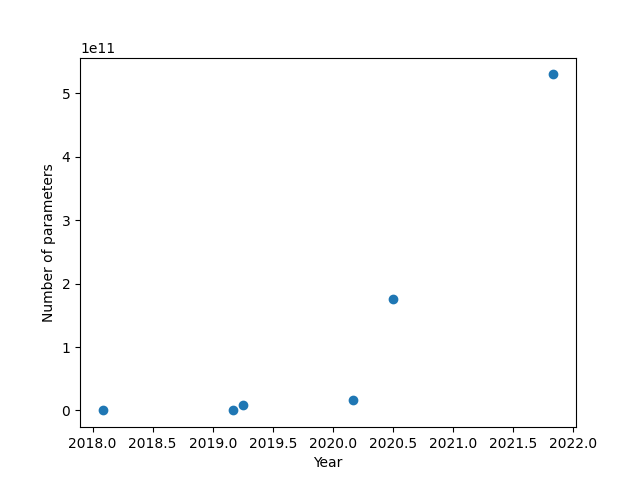
\includegraphics[width=\linewidth]{1b.png}
                \label{fig:rapport}    
                \caption{Uppgift: 1b}
            \end{figure}


            \begin{table} [h]
                \centering
                \caption{Uppgift 1c}
                \begin{tabular}{ | c | c |}
                    \hline
                    {\bf Uppgift 1c} & {\bf Number of parameters}  \\
                    \hline
                    1 & $log(94*10^6)$  \\
                    \hline
                    14 & $log(1.5*10^9)$  \\
                    \hline
                    15 & $log(8.3*10^9)$  \\
                    \hline
                    26 & $log(17*10^9)$  \\
                    \hline
                    30 & $log(175*10^9)$  \\
                    \hline
                    46 & $log(530*10^9)$  \\
                    \hline
                \end{tabular}
            \end{table}
        
            \begin{figure} [h]
                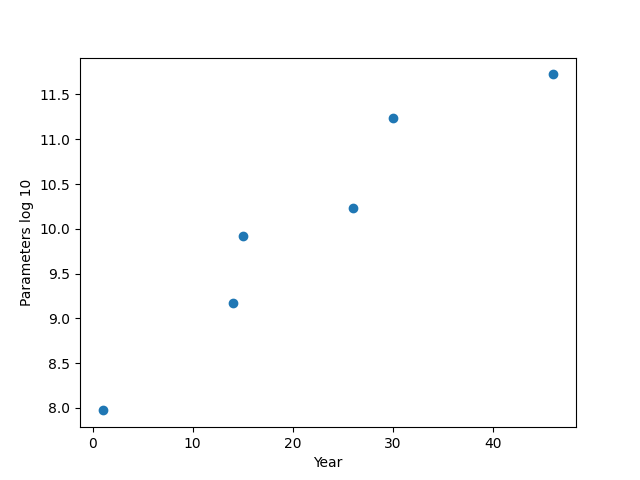
\includegraphics[width=\linewidth]{1c.png}   
                \caption{Uppgift: 1d}
            \end{figure}

            \begin{figure} [h]
                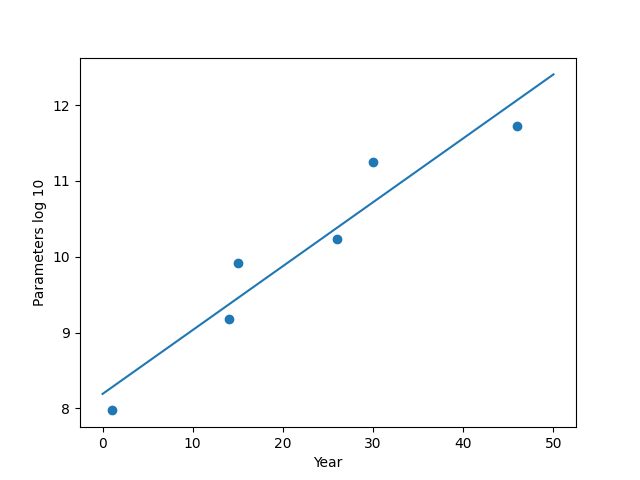
\includegraphics[width=\linewidth]{2c.png}
                \label{fig:rapport}    
                \caption{Uppgift: 2c}
            \end{figure}

            \begin{figure} [h]
                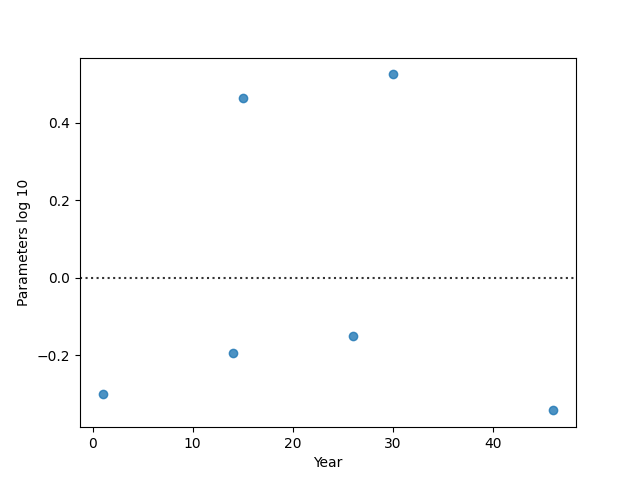
\includegraphics[width=\linewidth]{2d.png}
                \label{fig:rapport}    
                \caption{Uppgift: 2d}
            \end{figure} 

 \begin{figure} [h]
    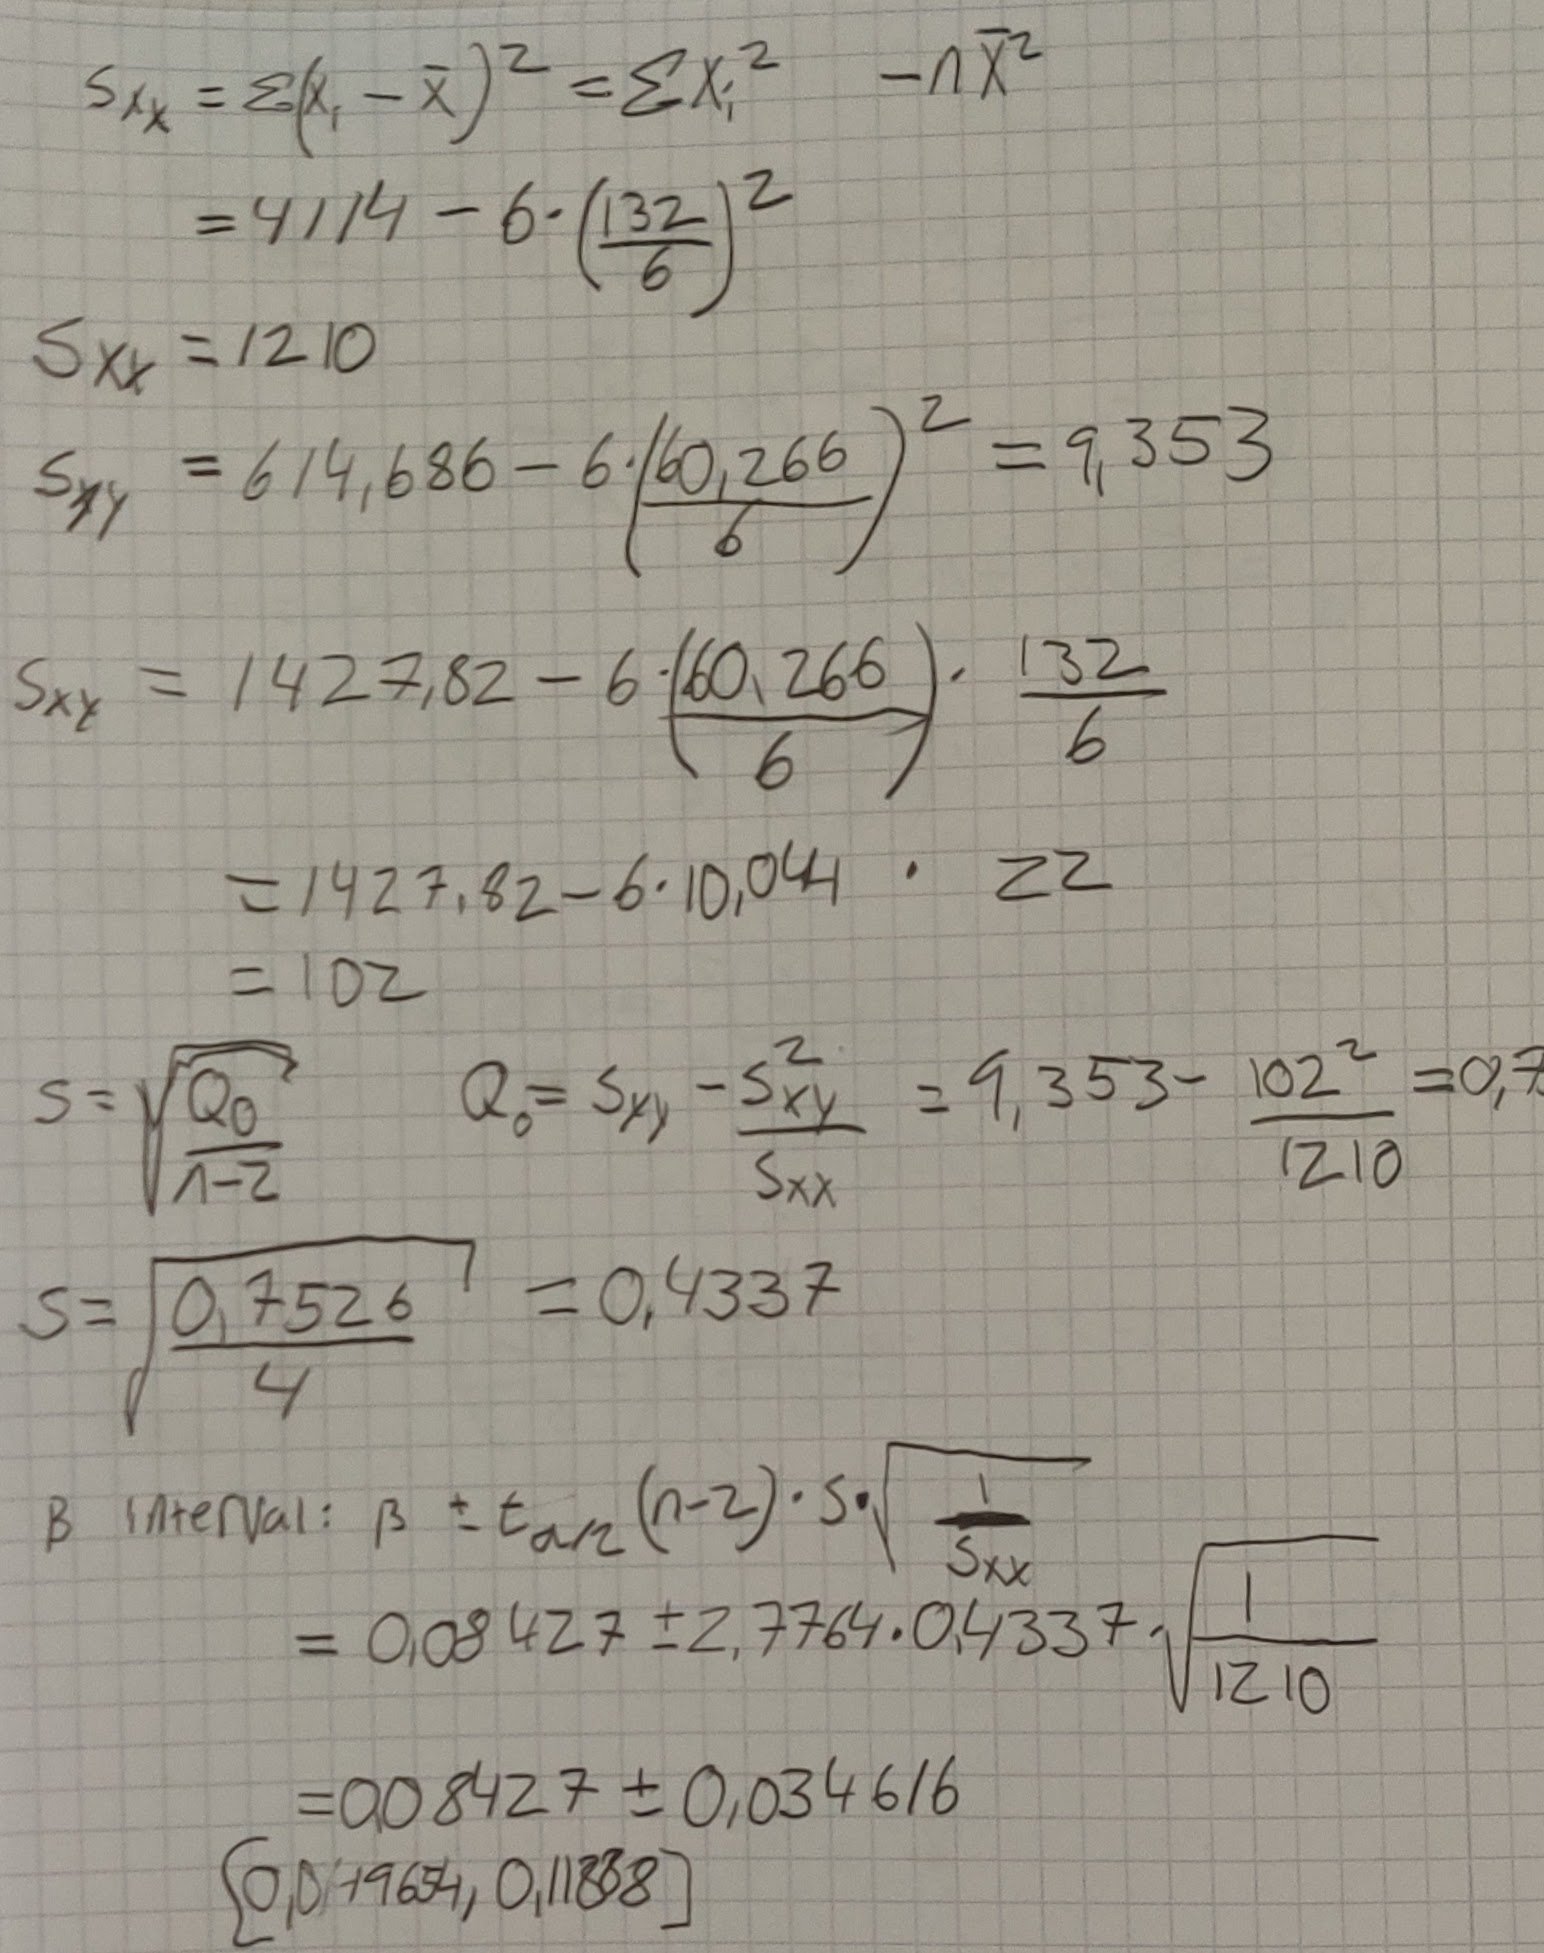
\includegraphics[width=\linewidth]{3a.jpg}   
    \caption{Uppgift: 3a}
\end{figure}

\begin{figure} [h]
    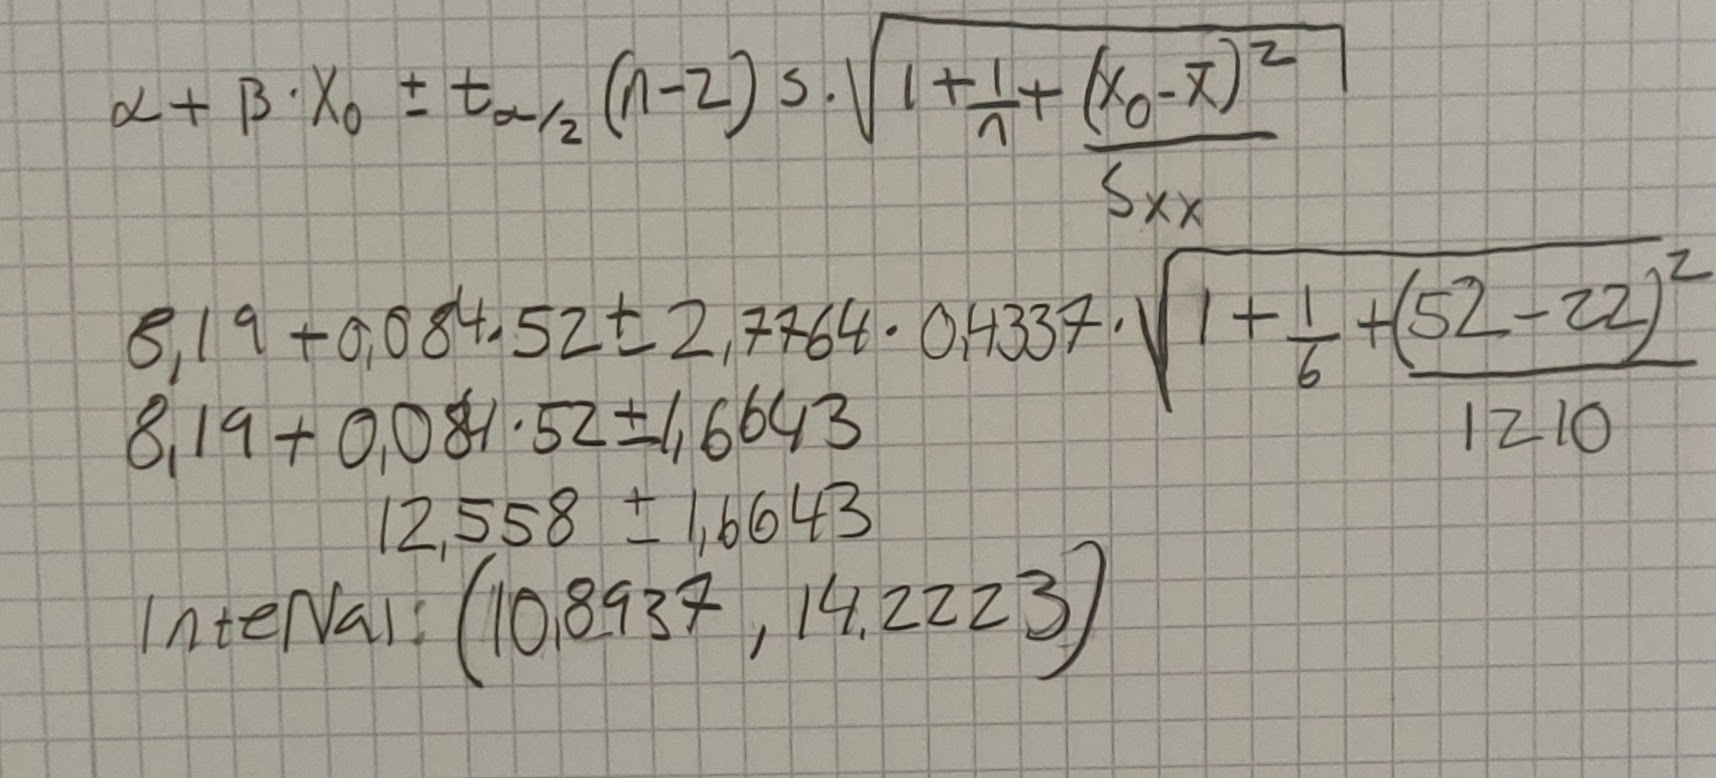
\includegraphics[width=\linewidth]{3b.jpg}   
    \caption{Uppgift: 3b}
\end{figure}
\end{document}